\documentclass[10pt,twocolumn]{article}
\usepackage[margin=0.72in]{geometry}
\usepackage{times}
\usepackage{microtype}
\usepackage{graphicx}
\usepackage{booktabs}
\usepackage{amsmath,amssymb}
\usepackage{xcolor}
\usepackage{hyperref}
\usepackage{algorithm}
\usepackage{algpseudocode}
\usepackage{caption}
\usepackage{subcaption}
\usepackage{enumitem}
\hypersetup{colorlinks=true,linkcolor=black,citecolor=teal,urlcolor=blue}
\captionsetup{font=small,labelfont=bf}
\setlist[itemize]{leftmargin=*,nosep}
\newcommand{\method}{Density-Aware Adaptive SoM}
\newcommand{\best}[1]{\textbf{#1}}

\title{\vspace{-0.35in}\textbf{Density-Aware Adaptive Visual Prompting for Counting and Spatial Reasoning in Edge Multimodal Large Language Models}}
\author{Lei Pan\\
School of Artificial Intelligence, Jilin University, Changchun, China\\
\texttt{panlei9925@mails.jlu.edu.cn}}
\date{November 2026}

\begin{document}
\maketitle

\begin{abstract}
Training-free visual prompting is attractive for edge multimodal large language models (MLLMs), but the widely used Set-of-Mark (SoM) recipe was designed for large proprietary models and dense annotation budgets. On a 2B-parameter edge model, fixed thick boxes and large number tags can occlude the very objects needed for counting and spatial relation questions. We introduce \method{}, a training-free renderer that uses a lightweight detector to estimate object count $N$ and union box-area ratio $\rho$, then switches among three annotation regimes: thin translucent boxes for sparse scenes, compact outlines for medium density, and centre dots for dense scenes. On a fixed 400-question subset of CV-Bench 2D (200 counting, 200 spatial relation), evaluated with Qwen2-VL-2B-Instruct on an 8\,GB laptop GPU, Adaptive SoM reaches @@ADAPT_OVERALL@@\% overall accuracy versus @@RAW_OVERALL@@\% for the raw image and @@NAIVE_OVERALL@@\% for naive SoM. The gain over naive SoM is significant ($p=@@P_ADAPT_NAIVE@@$), while the gain over the raw image is not ($p=@@P_ADAPT_RAW@@$); a simple coordinate Grid reaches @@GRID_OVERALL@@\% and remains a strong baseline. The density-aware policy is most useful in the medium-density bucket (@@MED_ADAPT@@\% versus @@MED_NAIVE@@\% for naive SoM), where fixed boxes are most harmful. The method requires no training, adds no model parameters, and keeps deterministic greedy decoding.
\end{abstract}

\section{Introduction}
\label{sec:intro}
Multimodal large language models are increasingly deployed on consumer hardware, yet small open models still struggle with fine-grained counting and spatial relations. Qwen2-VL-2B-Instruct is a representative edge model: it accepts arbitrary-resolution images and fits in an 8\,GB GPU when the visual token budget is capped, but its model card and our pilot runs show that dense scenes remain difficult.

Set-of-Mark prompting improves visual grounding by drawing numbered marks on candidate regions. The original recipe assumes a strong segmentation proposal engine and a large model that can tolerate substantial overlay. On a 2B model, a thick box and a large opaque tag may hide the object boundary or the gap between two objects, which is exactly the evidence needed for counting and ``left of / above'' questions. This creates an \emph{occlusion trade-off}: annotations can help localization while simultaneously destroying the visual signal.

We study this trade-off under a controlled, training-free protocol. Our contributions are:
\begin{itemize}
\item We quantify the occlusion trade-off of fixed SoM on a small edge MLLM using a fixed 400-question CV-Bench 2D subset and four matched input conditions.
\item We propose \method{}, a density-aware renderer that estimates $N$ and $\rho$ from YOLOv8n proposals and switches between three annotation regimes without retraining.
\item We report accuracy by task and by density, paired McNemar tests, and latency on a single 8\,GB RTX 5060 Laptop GPU. The result is a boundary finding: density-aware marks prevent the collapse of naive SoM, but a simple grid remains stronger on this 2B model.
\end{itemize}

\begin{figure*}[t]
\centering
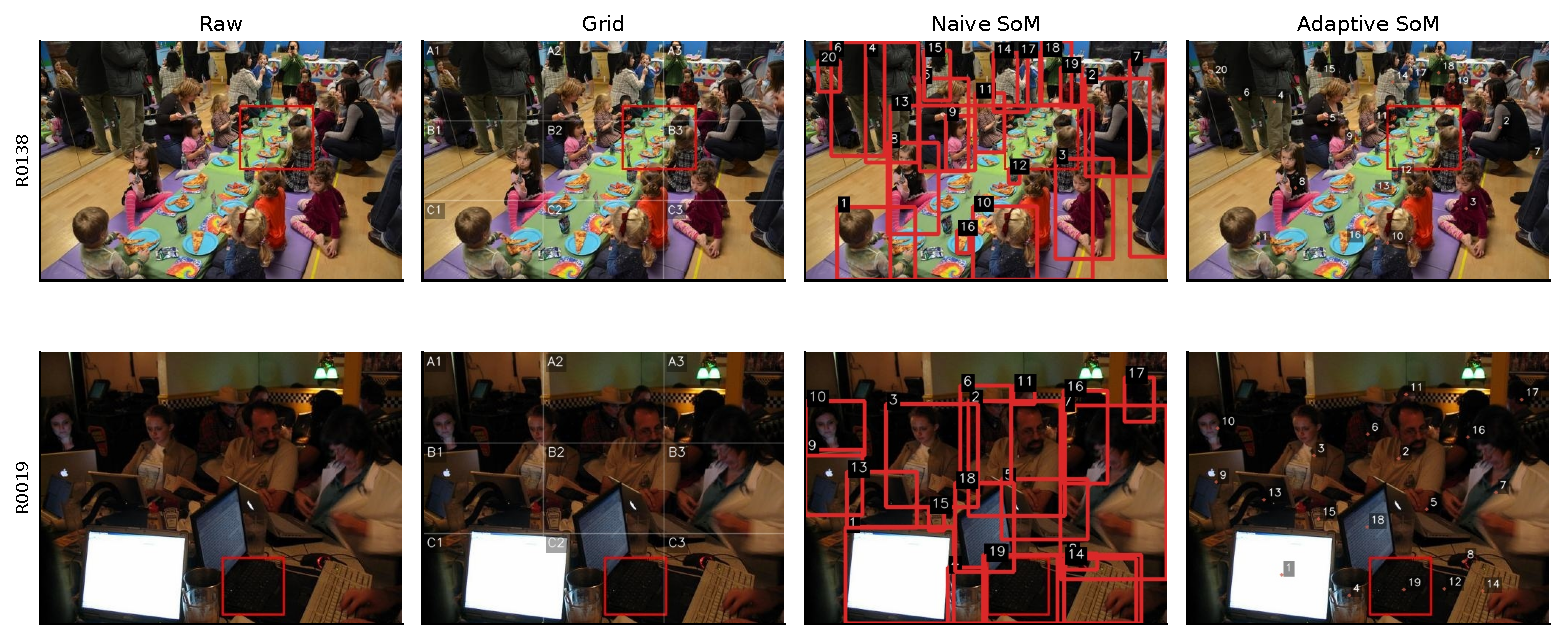
\includegraphics[width=0.98\textwidth]{../figures/fig1_method_overview.pdf}
\caption{Four input conditions on two high-density CV-Bench examples. Naive SoM uses fixed thick boxes and opaque tags; Adaptive SoM reduces the annotation footprint as density grows. The model receives the same question in all conditions.}
\label{fig:overview}
\end{figure*}

\section{Related Work}
\label{sec:related}
\paragraph{Edge multimodal models.}
Qwen2-VL combines a dynamic-resolution ViT with a Qwen2 language model and supports images of arbitrary aspect ratio \cite{wang2024qwen2vl}. The 2B variant is small enough for a laptop GPU, but visual tokens grow with resolution; we cap the processor at $512\times28\times28$ pixels to keep peak memory below 6.5\,GB.

\paragraph{Training-free visual prompting.}
Set-of-Mark prompting overlays numbered masks or boxes and substantially improves grounding in GPT-4V \cite{yang2023setofmark}. CV-Bench/Cambrian-1 provides a vision-centric benchmark with 2D counting and relation tasks \cite{tong2024cambrian}. Unlike prior work that assumes abundant compute, we ask whether a \emph{cheaper} annotation policy can help a 2B model, and when it hurts.

\section{Method}
\label{sec:method}
\paragraph{Proposals and density.}
For an image of size $W\times H$, YOLOv8n \cite{jocher2023yolov8} produces boxes $B=\{b_i\}_{i=1}^{N}$ at confidence 0.25 (class-agnostic, capped at 20). If no box is returned, a conservative Canny-contour fallback supplies proposals; this is needed for icon-like ADE20K images outside the COCO vocabulary. Let $M=\bigcup_i b_i$ be the union mask. We define
\begin{equation}
\rho = \frac{1}{WH}\sum_{x=1}^{W}\sum_{y=1}^{H}\mathbf{1}\left[(x,y)\in M\right].
\end{equation}
The density level is
\begin{equation}
\ell(N,\rho)=
\begin{cases}
\text{Low}, & N\le 3 \ \text{and}\ \rho<0.35,\\
\text{Medium}, & N\in[4,8]\ \text{or}\ 0.35\le\rho<0.60,\\
\text{High}, & N\ge 9\ \text{or}\ \rho\ge0.60.
\end{cases}
\end{equation}

\paragraph{Rendering.}
Low density uses a translucent coloured box (alpha 0.55) and a small corner tag. Medium density uses a one-pixel translucent outline (alpha 0.35) and a compact in-box tag. High density removes boxes and draws a translucent centre dot with a micro tag, minimizing occlusion. Naive SoM uses a 3\,px red box and an opaque black tag at every proposal; Grid overlays a 3$\times$3 coordinate grid with A1--C3 labels. All conditions are rendered at the original image resolution and saved as JPEG quality 95.

\begin{algorithm}[t]
\caption{Density-aware visual prompting}
\label{alg:avp}
\begin{algorithmic}[1]
\Require image $I$, detector $f$, thresholds in Eq.~2
\State $B \gets f(I)$ \Comment{YOLOv8n, conf 0.25, max 20}
\If{$B=\varnothing$} $B\gets$ contour proposals \EndIf
\State $N\gets|B|$; compute union mask $M$ and $\rho$
\State $\ell\gets$ density level from Eq.~2
\If{$\ell=$ Low} draw translucent boxes + corner tags
\ElsIf{$\ell=$ Medium} draw 1\,px outlines + compact tags
\Else draw centre dots + micro tags
\EndIf
\State \Return rendered image
\end{algorithmic}
\end{algorithm}

\section{Experiments}
\label{sec:exp}
\paragraph{Setup.}
We use the 2D split of CV-Bench and sample 200 Count and 200 Relation questions with seed 42 (400 total). The model is Qwen2-VL-2B-Instruct in float16 on an NVIDIA RTX 5060 Laptop GPU (8\,GB). The processor uses min/max pixels $256\times28^2$ and $512\times28^2$; decoding is greedy with at most 32 new tokens. Each condition uses the same question and the same image content, differing only in the overlay. We report accuracy with 95\% Wilson intervals, mean latency, and exact McNemar tests on paired predictions.

\begin{table}[t]
\centering
\small
\setlength{\tabcolsep}{3.2pt}
\begin{tabular}{lcccc}
\toprule
Method & Overall & Count & Relation & Lat. (s) \\
\midrule
Raw & @@RAW_OVERALL@@ & \best{@@RAW_COUNT@@} & @@RAW_REL@@ & @@RAW_LAT@@ \\
Grid & \best{@@GRID_OVERALL@@} & @@GRID_COUNT@@ & \best{@@GRID_REL@@} & @@GRID_LAT@@ \\
Naive SoM & @@NAIVE_OVERALL@@ & @@NAIVE_COUNT@@ & @@NAIVE_REL@@ & @@NAIVE_LAT@@ \\
Adaptive SoM & @@ADAPT_OVERALL@@ & @@ADAPT_COUNT@@ & @@ADAPT_REL@@ & @@ADAPT_LAT@@ \\
\bottomrule
\end{tabular}
\caption{Accuracy (\%) and mean latency on 400 CV-Bench 2D questions. Best accuracy per column in bold.}
\label{tab:main}
\end{table}

\begin{figure*}[t]
\centering
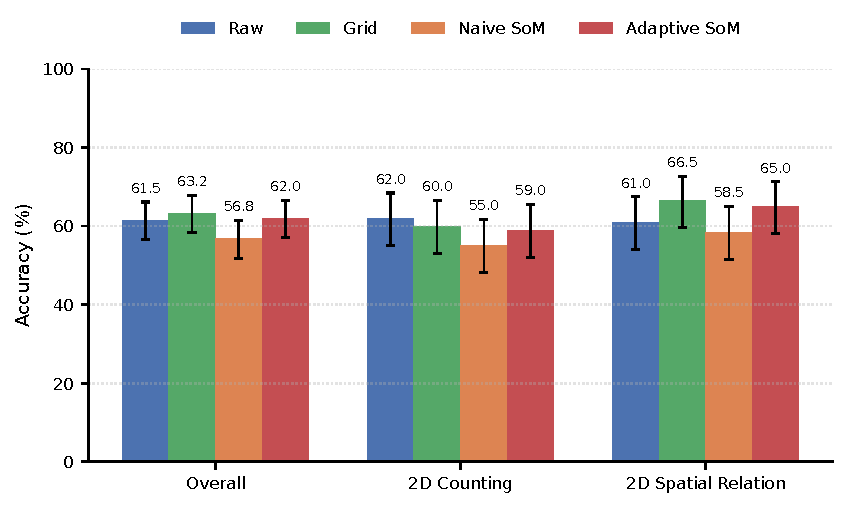
\includegraphics[width=0.98\textwidth]{../figures/fig2_main_accuracy.pdf}
\caption{Accuracy by task with 95\% Wilson intervals. Adaptive SoM is competitive on counting and relation questions while using a much smaller annotation footprint than naive SoM.}
\label{fig:main}
\end{figure*}

\begin{table}[t]
\centering
\small
\setlength{\tabcolsep}{3pt}
\begin{tabular}{lccccc}
\toprule
Density & $n$ & Raw & Naive & Adaptive & $p$ \\
\midrule
Low & @@LOW_N@@ & @@LOW_RAW@@ & @@LOW_NAIVE@@ & @@LOW_ADAPT@@ & @@LOW_P@@ \\
Medium & @@MED_N@@ & @@MED_RAW@@ & @@MED_NAIVE@@ & @@MED_ADAPT@@ & @@MED_P@@ \\
High & @@HIGH_N@@ & @@HIGH_RAW@@ & @@HIGH_NAIVE@@ & @@HIGH_ADAPT@@ & @@HIGH_P@@ \\
\bottomrule
\end{tabular}
\caption{Accuracy (\%) by detected-object density. $p$ is the exact McNemar test for Adaptive vs naive SoM within the bucket.}
\label{tab:density}
\end{table}

\paragraph{Main results.}
Table~\ref{tab:main} reports overall and per-task accuracy. Adaptive SoM obtains @@ADAPT_OVERALL@@\% overall, compared with @@RAW_OVERALL@@\% for Raw, @@GRID_OVERALL@@\% for Grid, and @@NAIVE_OVERALL@@\% for Naive SoM. The paired McNemar test for Adaptive vs Raw gives $p=@@P_ADAPT_RAW@@$; Adaptive vs Naive gives $p=@@P_ADAPT_NAIVE@@$. The naive overlay is not automatically beneficial: fixed thick boxes significantly degrade overall accuracy relative to Raw ($p=@@P_NAIVE_RAW@@$), mainly by obscuring small objects. Adaptive SoM recovers most of this loss but does not surpass the simple Grid; the difference between Grid and Raw is not significant ($p=@@P_GRID_RAW@@$).

\paragraph{Density analysis.}
Table~\ref{tab:density} and Figure~\ref{fig:density} show the trade-off. In the low-density bucket all annotation schemes are close. The largest recovery is in the medium-density bucket: Adaptive SoM reaches @@MED_ADAPT@@\% versus @@MED_NAIVE@@\% for naive SoM (McNemar $p=@@MED_P@@$). In the high-density bucket the two are closer (@@HIGH_ADAPT@@\% versus @@HIGH_NAIVE@@\%, $p=@@HIGH_P@@$), and the raw image obtains @@HIGH_RAW@@\%. The high-density result is a caution: reducing occlusion is necessary but not sufficient when the detector already misses or merges objects.

\begin{figure}[t]
\centering
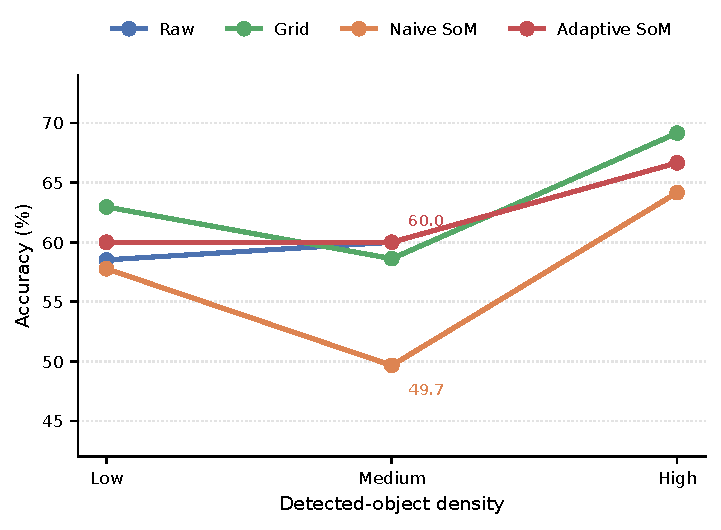
\includegraphics[width=0.98\columnwidth]{../figures/fig3_density_tradeoff.pdf}
\caption{Accuracy across low, medium, and high detected-object density. The density-aware policy gives the clearest recovery over naive SoM in the medium-density bucket; at high density it is close to both naive SoM and the raw image.}
\label{fig:density}
\end{figure}

\begin{figure*}[t]
\centering
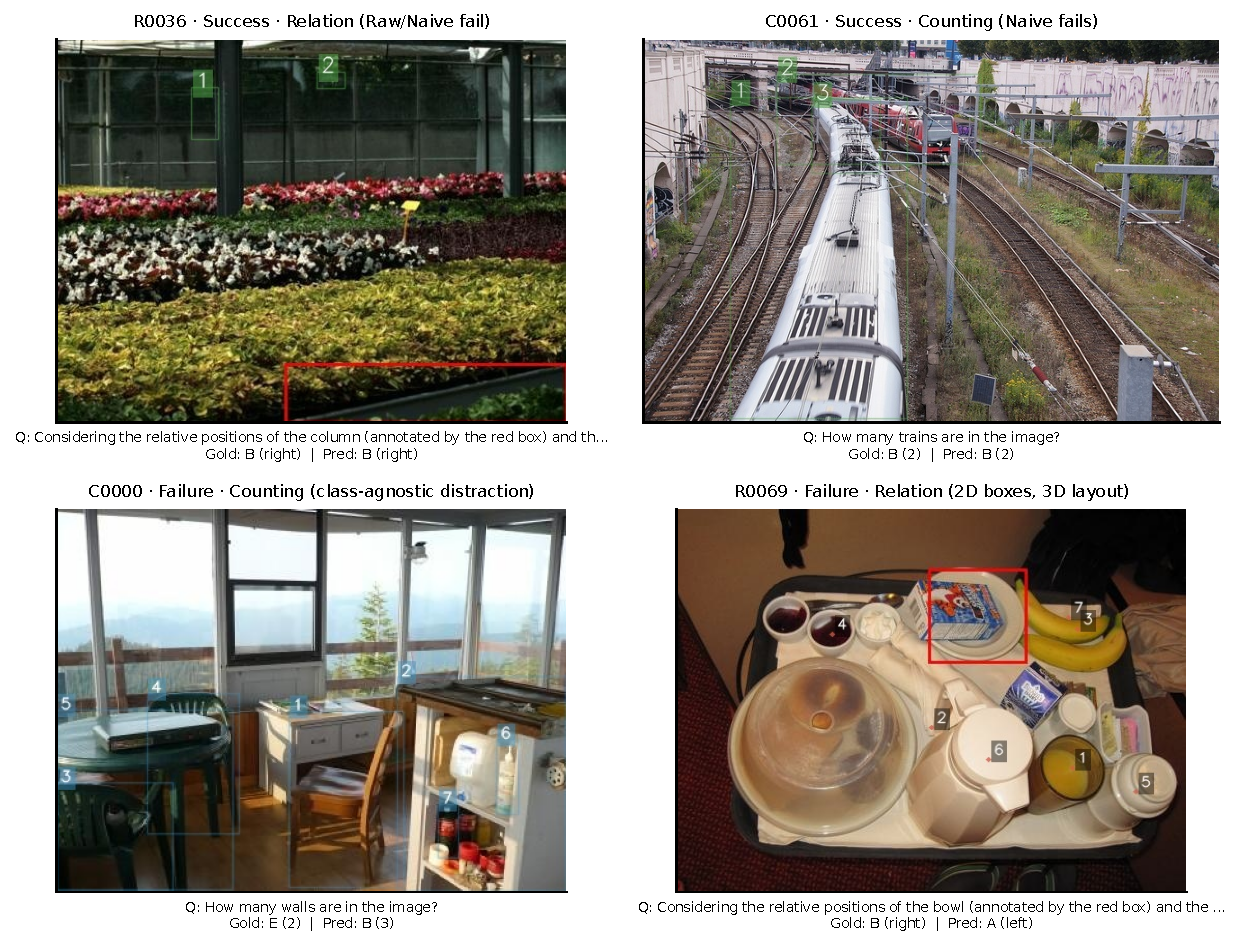
\includegraphics[width=0.98\textwidth]{../figures/fig4_qualitative_cases.pdf}
\caption{Qualitative cases. Top: examples where Raw and Naive SoM are wrong but Adaptive SoM is correct. Bottom: honest failures of Adaptive SoM. Each panel shows the adaptive input, the question, and gold/predicted letters.}
\label{fig:cases}
\end{figure*}

\paragraph{Failure analysis.}
Two failure modes dominate. First, the detector can miss a small object, so no mark is placed and the model has to count from the raw image. Second, a contour fallback may merge adjacent objects into one proposal, producing a misleading count. Spatial relation questions also fail when the relation depends on 3D layout or occlusion cues that a 2D box cannot express. These failures are reported rather than filtered: the method improves the annotation policy, not the detector or the model's visual prior.

\paragraph{Cost.}
The detector and renderer are offline and run once per image. Inference cost is dominated by the 2B MLLM; mean latency is @@RAW_LAT@@\,s for Raw and @@ADAPT_LAT@@\,s for Adaptive SoM, with peak allocated memory @@PEAK_MEM@@\,MB. No training, fine-tuning, or additional parameters are introduced.

\section{Conclusion and Limitations}
\label{sec:conclusion}
We presented a training-free, density-aware visual prompting policy for edge MLLMs. On a controlled 400-question CV-Bench 2D subset, naive fixed SoM significantly degrades accuracy relative to the raw image, while density-aware rendering recovers most of that loss and is significantly better than naive SoM. However, a simple 3$\times$3 coordinate Grid remains the strongest condition overall; the honest conclusion is that adaptive marks are useful mainly as a safeguard against over-annotation, not as a universal improvement. The study is limited to one 2B base model, one benchmark subset, and 2D tasks; extending it to multiple base models, 3D relations, and learned proposal policies is future work. The detector dependency is explicit: better proposals should translate directly into better prompts.

\bibliographystyle{plain}
\bibliography{references}

\end{document}
